\utsection{Analyse der Handover}{Thomas Waldecker}\label{sec:analyse}

\subsection{Vorbereitung}
\subsubsection{Tracen auf dem Um Interface mit einem Nokia 3310}\label{sec:umtrace}
Das Um Interface kann mit einem Nokia 3310 Mobiltelefon und einem dazugehörigen Adapter, der zwischen den Akku und das Telefon gesteckt wird und auf die vier Kontakte des internen Telefonbus zugreift getraced werden.

\begin{figure}[htbp]
	\centering
		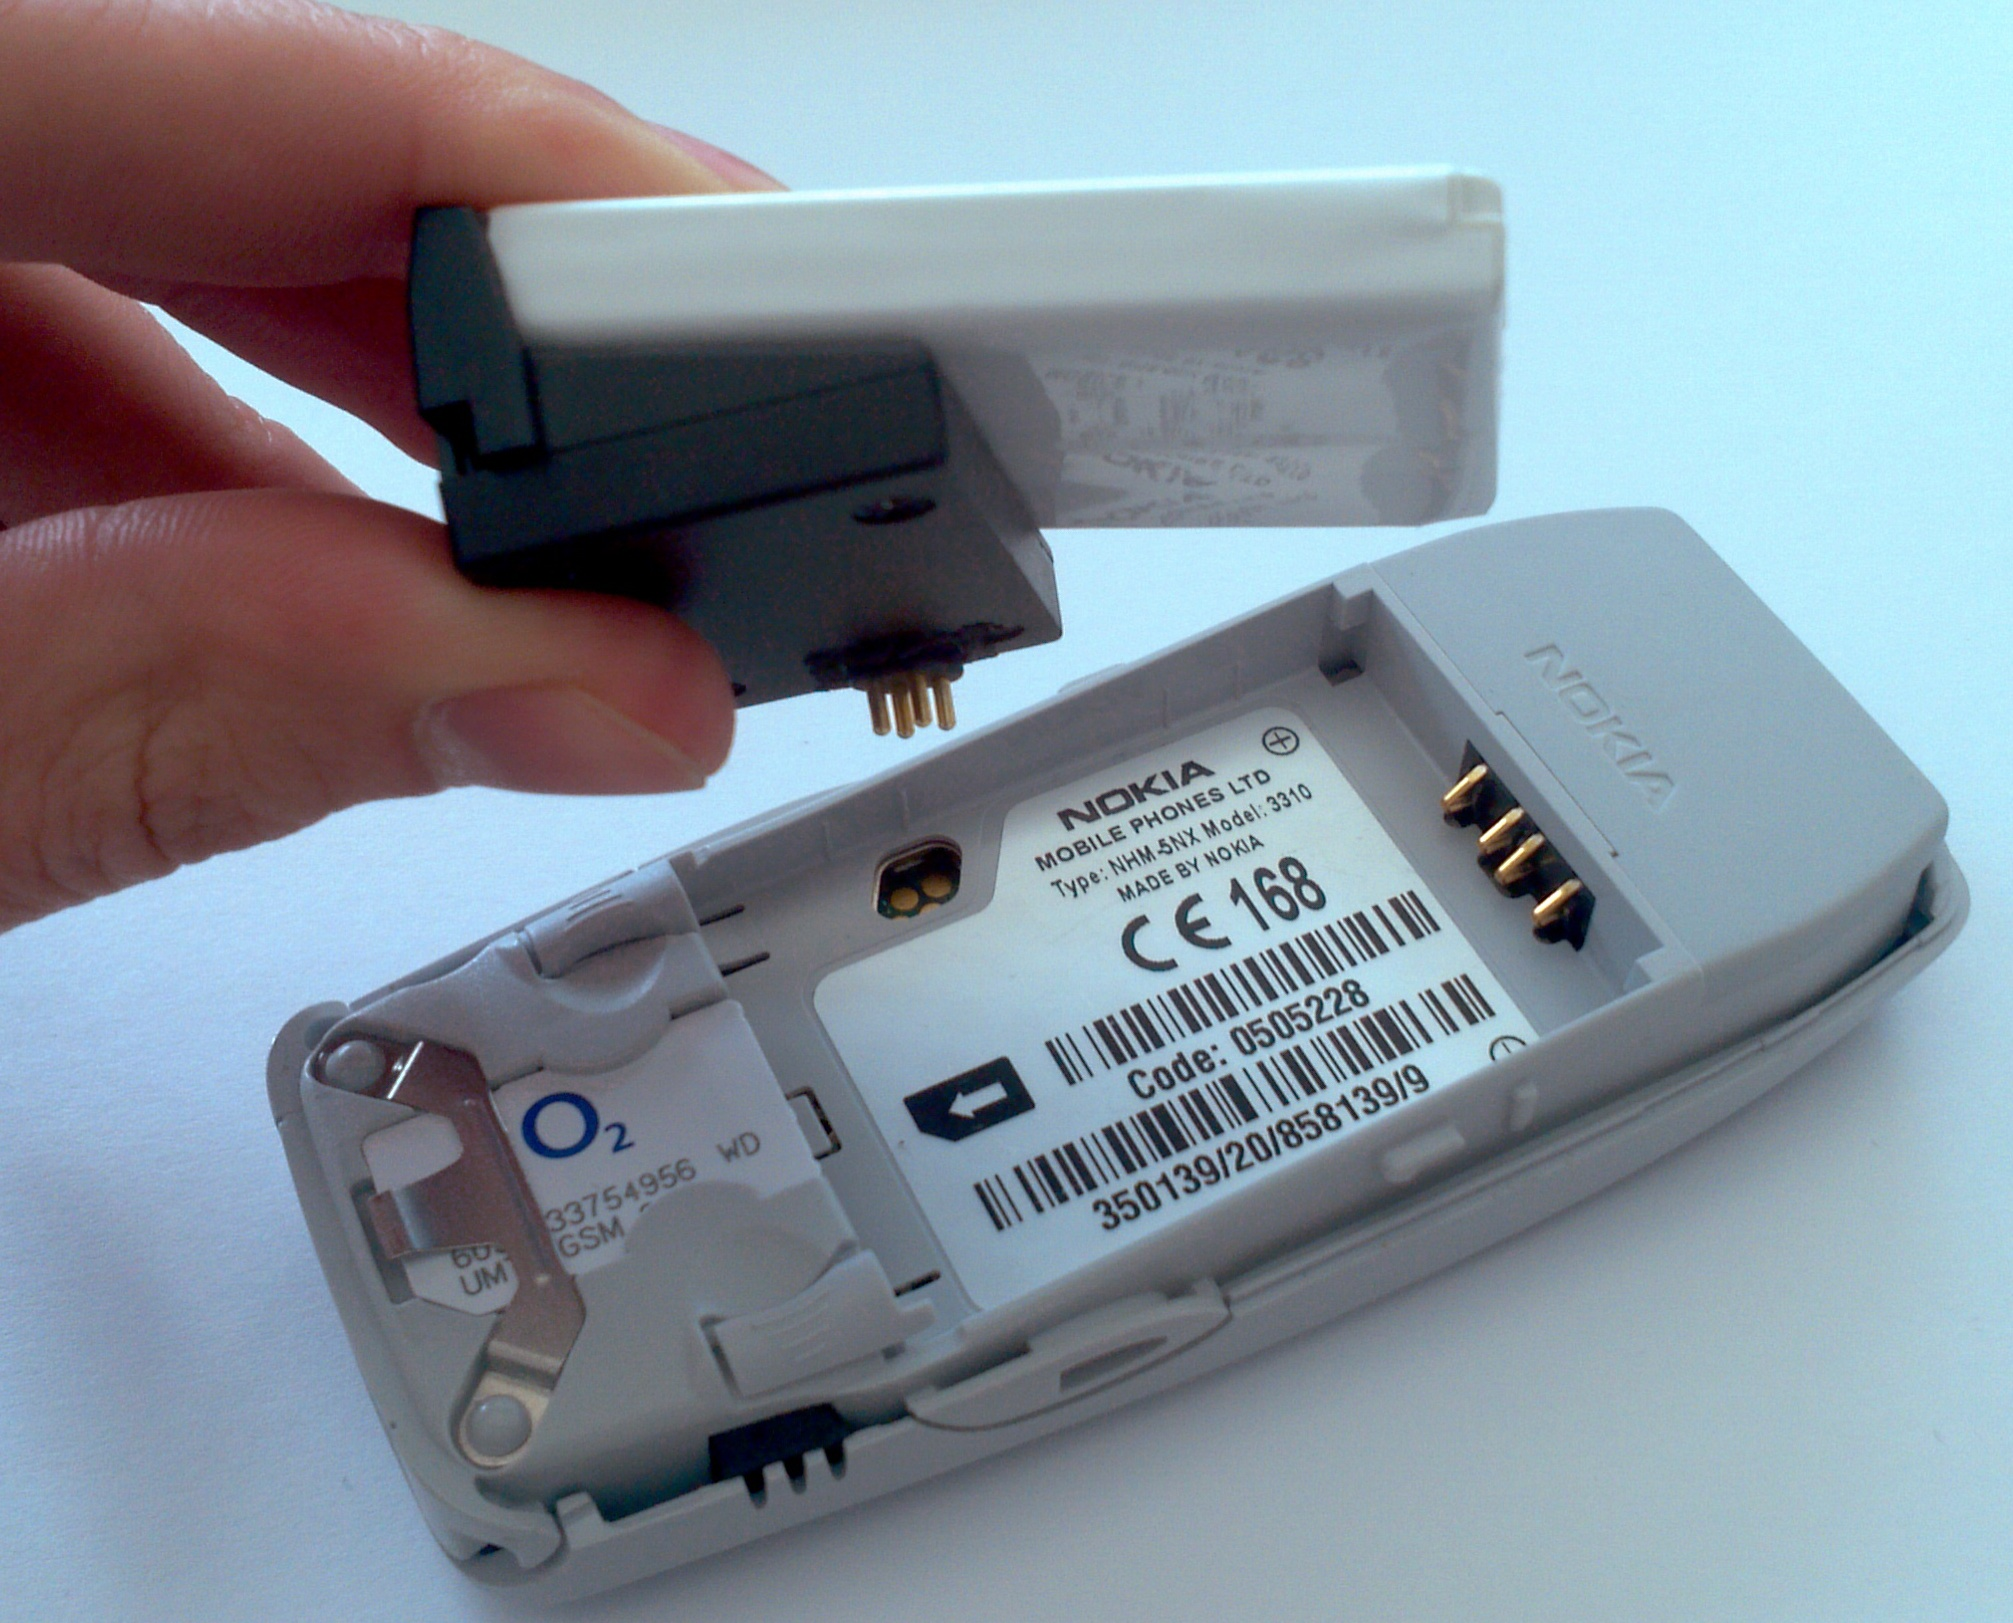
\includegraphics[width=0.6\textwidth]{img/nokia-trace}
	\caption{Adapter für ein Nokia 3310 um das Um Interface zu tracen}
	\label{fig:nokia-trace}
\end{figure}

Im Adapterkabel ist ein USB-zu-Seriell Wandler integriert. In die Konfigurationsdatei muss deshalb das Device des USB-Seriell Wandlers eingetragen werden (Siehe Listing \ref{config:gammu}).

\begin{lstlisting}[label=config:gammu,caption={Konfigurationsdatei für gammu und dem verwendeten Adapter}]
[gammu]

port = /dev/ttyUSB0
model = 6110
connection = mbus
synchronizetime = yes
logfile = 
logformat = nothing
use_locking = yes
gammuloc = 
\end{lstlisting}

Das Tracen kann nach der weiteren Konfiguration, die in \cite{bib:nokiagammu} beschrieben ist mit folgenden Kommando gestartet werden (Siehe Listing \ref{command:gammu}).

\begin{lstlisting}[label=command:gammu,caption={Aufruf von Gammu}]
sudo gammu --nokiadebug nhm5_587.txt v20-25,v18-19
Debug Trace Mode -- wumpus 2003
Loading
Activating ranges:
  20-25 verbose=1
  18-19 verbose=1
Debug Trace Enabled
Press Ctrl+C to interrupt...
<1805> MDI:m2d/FROM_MCU_TO_FBUS
t=0002 nr=0f: D 05: 1e 0c 00 40 00 06 01 01 70 01 01 47 
<198E> MDI:d2m/FROM_FBUS_TO_MCU
t=0003 nr=10: D 8E: 1e 00 0c 7f 00 02 40 07 
\end{lstlisting}

\subsubsection{Abis over IP tracen mit Wireshark}\label{sec:abistrace}
Das Abis Interface zwischen den \gls{bts} und dem \gls{bsc} kann mit Wireshark getraced werden (Siehe Abbildung \ref{fig:openbscarch}). Dazu wird auf der Maschine auf der OpenBSC läuft Wireshark auf dem Ethernet-Interface gestartet.

Das Abis over IP Protokoll wird nicht von Wireshark unterstützt und aufgelöst. Dieses Feature steht aber als Patches für Wireshark vom OpenBSC Projekt zur Verfügung.

Die Patches für Wireshark liegen im Repository von OpenBSC. Die Doku im OpenBSC-wiki ist dafür nicht so hilfreich. Wenn man sich den Quelltext von OpenBSC holt sind im Verzeichnis \lstinline{wireshark/} verschiedene Patches die auf die SVN-Revision r38894 von Wireshark angewendet werden können. Damit werden verschiedene Features zu Wireshark hinzugefügt \cite{bib:wiresharkabis, bib:wiresharkabisreadme}.

Angewendet werden diese Patches mit folgendem Kommando (ausgeführt im Wireshark Quelltextverzeichnis mit SVN Revision r38894):
\begin{lstlisting}[caption={Patchen von Wireshark}]
$ patch -p1 < $OPENBSC_DIR/wireshark/0001-abis_oml.patch
$ patch -p1 < $OPENBSC_DIR/wireshark/0002-ericsson_rbs2409.patch
$ patch -p1 < $OPENBSC_DIR/wireshark/0003-lucent-hnb.patch
$ patch -p1 < $OPENBSC_DIR/wireshark/0004-rsl-ipaccess.patch
$ patch -p1 < $OPENBSC_DIR/wireshark/0005-rsl-hsl.patch
$ patch -p1 < $OPENBSC_DIR/wireshark/0006-abis_oml-hsl.patch 
\end{lstlisting}

\subsection{Intra BSC Handover mit OpenBSC und zwei nanoBTS}

\subsubsection{Aufbau und Durchführung}
In einem Raum (Mobile Netze Labor) wurde an zwei Ecken jeweils eine nanoBTS gelegt und per Ethernet mit dem Laborrechner verbunden. Auf dem Rechner wurde OpenBSC gemäß Kapitel \ref{sec:openbsc} konfiguriert. Durch hin und hergehen zwischen den beiden \gls{bts} während eines Anrufs soll das OpenBSC Handover auslösen.

Während des Anrufs wurde das Um Interface (siehe Kapitel \ref{sec:umtrace}) und das Abis Interface (siehe Kapitel \ref{sec:abistrace}) getraced um die Handover aufzunehmen.

Abbildung \ref{fig:adhandover} zeigt das Ablaufdiagramm eines Handovers. In den Folgenden zwei Abschnitten werden die zwei Traces untersucht. 

\subsubsection{Ablauf Handover auf dem Um Interface}\label{sec:obsc-um}

Während eines Anrufs werden laufend \textit{Measurement Reports} an die \gls{bts} über den \gls{sacch} gesendet. Die \gls{bts} leitet die Reports an die \gls{bsc} weiter, die letzendlich auch die Entscheidung über einen Handover trifft. Ist diese Entscheidung getroffen wird an die Mobilstation ein Handover Command gesendet. Die Mobilstation führt dann den Handover aus indem sie der neuen \gls{bts} eine \gls{sabm} Nachricht sendet um eine Verbindung aufzubauen. Die BTS beantwortet den \gls{sabm} Request mit einem \gls{UA} \cite[3.4.4]{bib:3gpp0408}\cite[3.1.5]{bib:3gpp0408} \cite[1.7.4]{bib:grundkursmks}.

Die in diesem Abschnitt aufgeführten Auszüge aus Tracefiles stammen aus der Datei \lstinline{files/openbsc-traces/handoversuccess.xml} in \cite{bib:githubfiles}.

Listing \ref{lst:bschandovertrace} zeigt die relevanten Pakete des Handovers auf dem Um Interface.

\begin{lstlisting}[label=lst:bschandovertrace,caption={Übersicht über die gesendeten Pakete auf dem Um Interface},numbers=none]
No. Src Dest Protocol Length Info
271	MS	BTS  LAPDm	  23     U, func=UI(DTAP) (RR) Measurement Report 
284	BTS	MS   LAPDm	  23     I, N(R)=4, N(S)=2(DTAP) (RR) Handover Command 
292	MS  BTS  LAPDm    23     U P, func=SABM
297	BTS MS   LAPDm	  23     U F, func=UA
\end{lstlisting}

Im weiteren Teil dieses Abschnitts wird auf die am Handover beteiligten Nachrichten genauer eingegangen.

\textbf{System Information Type 2}
Damit die Mobilstation erfährt welche benachbarten Zellen relevant sind für die Messung der Signalstärke schickt die Basisstation ein System Information Type 2. Diese benachbarten Zellen müssen vorher im BSC konfiguriert werden. In Listing \ref{lst:sysinftype2} ist ein Auszug aus dem System Information Type 2 mit dem die Neighbour Cell Description mitgesendet wird. Dort sieht man die List of \glspl{ARFCN}

\begin{lstlisting}[label=lst:sysinftype2,caption={Nachbarzellen im System Information Type 2}]
Neighbour Cell Description - BCCH Frequency List
..0. .... = EXT-IND: The information element carries the complete BA (0)
...0 .... = BA-IND: 0
10.. 111. = Format Identifier: variable bit map (0x47)
List of ARFCNs = 846
\end{lstlisting}

\textbf{Measurement Report}
Im Measurement Report sind die Measurement Results enthalten. Die Spezifikation mit dem Layout und der Beschreibung der Results ist in \cite[10.5.2.20]{bib:3gpp0408}. In Listing \ref{lst:measurement-result} ist die Beschreibung eines per Wireshark getraceten Reports abgedruckt.

Der Inhalt der Measurement Results wird nun kurz erklärt. Das Feld \lstinline{RXLEV-FULL-SERVING-CELL} gibt die empfangene Signalstärke auf allen Slots an. Das Messergebnis ist gültig, das gibt uns das Feld \lstinline{MEAS-VALID} an. Der Wert im Feld \lstinline{NO-NCELL} gibt an, das wir ein Messergebnis für eine Nachbarzelle haben. Das Messergebnis für dei Nachbarzelle ist im Feld \lstinline{RXLEV-NCELL} \cite[Table 10.40]{bib:3gpp0408}.

\begin{lstlisting}[label=lst:measurement-result,caption={Measurement Result}]
351	0	MS	BTS	LAPDm	23	U, func=UI(DTAP) (RR) Measurement Report 
  GSM A-I/F DTAP - Measurement Report
    Measurement Results
    0... .... = BA-USED: 0
    .0.. .... = DTX-USED: DTX was not used
    ..10 0010 = RXLEV-FULL-SERVING-CELL: -77 <= x < -76 dBm (34)
    0... .... = 3G-BA-USED: 0
    .0.. .... = MEAS-VALID: The measurement results are valid
    ..10 0100 = RXLEV-SUB-SERVING-CELL: -75 <= x < -74 dBm (36)
    .000 .... = RXQUAL-FULL-SERVING-CELL: BER < 0.2%, Mean value 0.14% (0)
    .... 000. = RXQUAL-SUB-SERVING-CELL: BER < 0.2%, Mean value 0.14% (0)
    .... ...0  01.. .... = NO-NCELL-M: 1 neighbour cell measurement result (1)
    ..10 1101 = RXLEV-NCELL: 45
    0000 0... = BCCH-FREQ-NCELL: 0
    .... .111  111. .... = BSIC-NCELL: 63
\end{lstlisting}

\textbf{Handover Command}
Fällt der \gls{bsc} die Entscheidung für einen Handover dann sendet die Basisstation einen Handover Command in dem unter anderem die Frequenz des Kontrollkanals (\gls{BCCH} \gls{ARFCN}) und die Beschreibung des \gls{TCH/F}, bestehend aus dem Timeslot und der Frequenz \gls{ARFCN}.

\begin{lstlisting}[label=lst:handover-command,caption={Handover Command}]
DTAP Radio Resources Management Message Type: Handover Command (0x2b)
 Cell Description
  ..11 1... = NCC: 7
  .... .111 = BCC: 7
  BCCH ARFCN(RF channel number): 840
 Channel Description 2 - Description of the first channel, after time
  0000 1... = TCH/F + FACCH/F and SACCH/F
  .... .010 = Timeslot: 2
  111. .... = Training Sequence: 7
  ...0 .... = Hopping channel: No
  .... 00.. = Spare
  Single channel : ARFCN 840
 Handover Reference
  Handover reference value: 6
 Power Command and access type
\end{lstlisting}

Nach dem Handover Command baut die Mobilstation eine neue Verbindung auf und fängt mit der Contention Resolution an. Dazu sendet sie ein SABM und bekommt als Antwort ein UA \cite[5.4.1.4]{bib:3gpp0406}.



\subsubsection{Handover auf der Abis Schnittstelle zwischen OpenBSC und den zwei nanoBTS}

Wie in Abbildung \ref{fig:adhandover} zu sehen ist bekommt der \gls{bsc} in unserem Fall OpenBSC von der \gls{bts} mit der aktiven Verbindung die Measurement Reports. Entscheidet sich der \gls{bsc} für einen Handover dann sendet er ein Channel Activation an die neue \gls{bts}. Diese allokiert einen neuen Kanal und antwortet dann mit einem Channel Activation Acknowledgement. Dann sendet der \gls{bsc} den Handover Command zur alten BTS. Sobald ein Established Indication von der neuen BTS eintrifft wird der Sprachkanal an die neue BTS umgeleitet. Am Ende wird der Kanal auf der alten BTS mit einem Channel Release freigegeben. Die BTS bestätigt dies mit einem Channel Release Acknowledgement.

Um das Abis Interface auf dem Rechner mit OpenBSC zu tracen wurde der Wireshark mit den Patches gepatcht und kompiliert (siehe Abschnitt \ref{sec:abistrace}). Um nur die relevanten Pakete anzuzeigen wurde im Wireshark auf die Dateien \lstinline{files/openbsc-traces/handover-abis} und \lstinline{files/openbsc-traces/handover-abis-part} aus \cite{bib:githubfiles} folgender Filter angewandt:

\begin{lstlisting}[numbers=none]
(ip.addr == 10.28.9.33 or ip.addr == 10.28.9.34) and (ip.proto != 17)
\end{lstlisting}

Dieser Filter zeigt nur die Pakete an die von einer der beiden nanoBTS empfangen oder gesendet werden. Außerdem werden alle Pakete die per UDP Protokoll gesendet werden ausgeblendet.

Wendet man diesen Filter an, erhält man eine gute Übersicht und kann die relevanten Abis-Pakete inspizieren. Listing \ref{lst:abis-trace} zeigt einen Auszug aus dem Tracefile in dem der oben erkärte Ablauf zu erkennen ist. Anzumerken ist noch das die IP-Adressen mit den Endungen 33 und 34 die nanoBTS sind.

\begin{lstlisting}[label=lst:abis-trace,caption={Abis Trace mit Handover Nachrichten}]
No Source     Dest.    Len. Info
29 10.28.9.34 10.28.9.31 96	MEASurement RESult (DTAP) (RR) Measurement Report 
31 10.28.9.31 10.28.9.33 85	CHANnel ACTIVation 
32 10.28.9.33 10.28.9.31 64	CHANnel ACTIVation ACKnowledge 
34 10.28.9.31 10.28.9.34 75	DATA REQuest (DTAP) (RR) Handover Command 
47 10.28.9.33 10.28.9.31 63	ESTablish INDication 
51 10.28.9.31 10.28.9.34 65	RELease REQuest 
54 10.28.9.34 10.28.9.31 63	RELease CONFirm 
56 10.28.9.31 10.28.9.34 61	RF CHANnel RELease 
57 10.28.9.34 10.28.9.31 61 RF CHANnel RELease ACKnowledge 
\end{lstlisting}

\subsection{Intra BTS Handover mit OpenBTS}
\subsubsection{Aufbau und Durchführung}
Auf dem Laborrechner wurde OpenBTS und Asterisk gemäß dem Kapitel \ref{sec:openbts} installiert und konfiguriert. Die Handoverfunktionalität wurde wie in Kapitel \ref{sec:erweiterung} beschrieben Implementiert. Der Quelltext der Erweiterung ist im github Repository \cite{bib:openbtshandover} öffentlich verfügbar. 

Mit einem Nokia Handy wurde der Echo-Test von Asterisk angerufen (siehe Kapitel \ref{sec:asterisk}). Das Um Interface wurde während des Anrufs mit dem Adapter (siehe Abschnitt \ref{sec:umtrace}) getraced. 

Um einen Handover auszulösen wurde in die Entscheidungslogik des Handovers ein Hack eingebaut (siehe Abschnitt \ref{sec:hom}), der dann einen Handover auslöst, wenn eine Datei im OpenBTS Verezichnis existiert.

Während eines laufenden Anrufs wurde diese Datei angelegt und damit der Handover durchgeführt. Die entstandenen Traces werden nun analysiert. Das entsprechende Tracefile ist \lstinline{files/openbts-traces/handover-test-b.xml}

\textbf{System Information Type 2} Als Nachbarzellen wurden die \glspl{ARFCN} 846 und 867 konfiguriert, wobei 867 die eigene Frequenz der Basisstation ist. Im Auszug des System Information Type 2 in Listing \ref{lst:obts-sysinft2} sind diese Informationen zu sehen.

\begin{lstlisting}[label=lst:obts-sysinft2, caption={Auszug aus dem System Information Type 2 von OpenBTS}]
Frame 104: 23 bytes on wire (184 bits), 23 bytes captured (184 bits)
GSM Um Interface
  ARFCN: 867
GSM A-I/F DTAP - System Information Type 2
  Neighbour Cell Description - BCCH Frequency List
    List of ARFCNs = 846 867
\end{lstlisting}

\textbf{Measurement Report} Es wurde keine Basisstation mit der \gls{ARFCN} 846 zu diesem Zeitpunkt betrieben. Im Measurement Report wird deshalb nur die \gls{bts} 1 (\lstinline{BCCH-FREQ-NCELL}) der Null-indizierten Liste des System Information Type 2 aufgeführt (vgl. das Measruement Report im OpenBSC Kapitel \ref{sec:obsc-um}). Diese ist die gleiche wie die aktuelle \gls{bts} und zeigt auch das gleiche Messergebnis 63.

\begin{lstlisting}[label=lst:obts-mmrept, caption={Auszug aus dem Measurement Report}]
Frame 168: 23 bytes on wire (184 bits), 23 bytes captured (184 bits)
GSM A-I/F DTAP - Measurement Report
  Measurement Results
    ..11 1111 = RXLEV-FULL-SERVING-CELL: >= -48 dBm (63)
    .0.. .... = MEAS-VALID: The measurement results are valid
    .... ...0  01.. .... = NO-NCELL-M: 1 neighbour cell measurement result (1)
    ..11 1111 = RXLEV-NCELL: 63
    0000 1... = BCCH-FREQ-NCELL: 1
    .... .000  010. .... = BSIC-NCELL: 2
\end{lstlisting}

\textbf{Handover Command} Der Handover wird über den Hack (siehe Abschnitt \ref{sec:hom}) getriggert. Die Basisstation sendet daraufhin das Handover Command in dem auch der neue Timeslot übergeben wird. 

\begin{lstlisting}[label=obtshoc, caption={Auszug aus dem Handover Command}]
Frame 209: 23 bytes on wire (184 bits), 23 bytes captured (184 bits)
GSM A-I/F DTAP - Handover Command
Channel Description 2 - Description of the first channel, after time
.... .110 = Timeslot: 6
\end{lstlisting}

Der Handover schlägt fehl, da der Traffic Channel nicht weitergeleitet wird. Die Mobilstation sendet deshalb Handover Failures und die BTS Disconnected daraufhin die Mobilstation.























